%=================================================================
% TrustMedX -- IEEE journal manuscript (IEEEtran)
% Compile: pdflatex -> bibtex -> pdflatex -> pdflatex
%=================================================================
\documentclass[12pt,onecolumn,journal]{IEEEtran}

\usepackage[utf8]{inputenc}
\usepackage[T1]{fontenc}
\usepackage{graphicx}
\usepackage{booktabs}
\usepackage{threeparttable}
\usepackage{array}
\usepackage{multirow}
\usepackage{amsmath,amssymb}
\usepackage{url}
\usepackage[hidelinks]{hyperref}
\usepackage{cite}

\begin{document}

\title{TrustMedX: A Trustworthy Clinical Decision Support Framework for 30-Day Diabetes Readmission Prediction}

\author{Satwik~Shreshth%
\thanks{S. Shreshth is with the TrustMedX Research Project (e-mail: satwikshreshth2002@gmail.com).}%
\thanks{Manuscript prepared July 2026. This work describes a research prototype; it is not a medical device and is not intended for clinical use.}}

\markboth{TrustMedX Research Project}{Shreshth: TrustMedX}

\maketitle

\begin{abstract}
Most machine learning research in clinical decision support reports predictive accuracy in isolation, without addressing whether clinicians can trust or act on a given prediction. Two gaps limit real-world adoption: predictions lack calibrated confidence, so a 51\%-confident and a 99\%-confident ``high risk'' flag are indistinguishable; and feature-attribution explanations are not grounded in verifiable clinical evidence. We present TrustMedX, a research-grade clinical decision support framework for predicting 30-day hospital readmission risk in diabetic patients that integrates calibrated uncertainty quantification and retrieval-grounded explanation alongside standard machine learning and explainable AI techniques. We evaluate 14 models on the Diabetes 130-US Hospitals dataset (101,766 encounters), finding that gradient-boosted tree models achieve the best discriminative performance (AUROC 0.6672, AUPRC 0.2201), consistent with published benchmarks on this task. Temperature scaling improves the expected calibration error from 0.3385 to 0.3257, split conformal prediction attains 0.8969 empirical coverage at a 90\% target, and SHAP analysis identifies prior inpatient utilization and discharge disposition as the dominant predictors. A red-team hallucination test demonstrates that the retrieval-augmented explanation engine declines to incorporate fabricated evidence rather than generating plausible but false justifications.
\end{abstract}

\begin{IEEEkeywords}
Clinical decision support, machine learning, explainable AI, uncertainty quantification, calibration, conformal prediction, retrieval-augmented generation, SHAP.
\end{IEEEkeywords}

\IEEEpeerreviewmaketitle

\section{Introduction}
\label{sec:introduction}
\IEEEPARstart{M}{achine} learning for clinical decision support has progressed substantially over the past decade, yet a fundamental limitation persists: most systems report discriminative accuracy in isolation, without measuring whether a clinician can trust or act on an individual prediction \cite{strack2014impact}. Two gaps limit real-world adoption. First, predictions frequently lack calibrated confidence: a model may attain a respectable area under the receiver operating characteristic curve (AUROC) while its probability estimates are systematically miscalibrated, so that a stated 70\% risk may correspond to a true frequency of 50\% or 90\% \cite{guo2017calibration}. Second, post-hoc explanation methods such as SHAP \cite{lundberg2017unified} and LIME \cite{ribeiro2016should} identify which input features contributed to a prediction but do not connect those features to verifiable clinical evidence.

TrustMedX addresses both gaps in a single, measurable, reproducible system for predicting 30-day hospital readmission in diabetic patients. The framework combines (i) a systematic comparison of 14 predictive models, (ii) probability calibration via temperature scaling \cite{guo2017calibration}, (iii) distribution-free uncertainty quantification via split conformal prediction \cite{vovk2005algorithmic,angelopoulos2021gentle}, (iv) global and per-patient explanation via SHAP \cite{lundberg2017unified}, and (v) retrieval-augmented synthesis of structured, cited explanations \cite{lewis2020retrieval} under an explicit constraint against fabricating unsupported claims.

The contributions of this paper are:
\begin{itemize}
    \item a comprehensive evaluation of 14 models, including gradient-boosted trees, neural networks, and ensembles, on the Diabetes 130-US Hospitals benchmark;
    \item integration of temperature scaling, conformal prediction, and bootstrap confidence intervals into a single readmission-risk pipeline;
    \item a retrieval-augmented explanation engine that combines SHAP attributions, calibrated confidence, and retrieved clinical evidence into structured, cited narratives;
    \item a red-team hallucination test demonstrating that the engine refuses to justify predictions with fabricated evidence; and
    \item a fairness analysis across race, gender, and age subgroups, identifying a clinically meaningful performance degradation in elderly patients.
\end{itemize}

The remainder of the paper is organized as follows. Section~\ref{sec:related} reviews related work. Section~\ref{sec:methods} describes the dataset and methods. Section~\ref{sec:results} presents experimental results. Sections~\ref{sec:discussion}--\ref{sec:limitations} discuss findings and limitations, Section~\ref{sec:ethics} states ethical considerations, and Section~\ref{sec:conclusion} concludes.

\section{Related Work}
\label{sec:related}
\subsection{Readmission Prediction}
Strack \emph{et al.} \cite{strack2014impact} introduced the Diabetes 130-US Hospitals dataset and reported baseline models relating HbA1c measurement to early readmission, establishing the dataset as a standard benchmark. Subsequent studies on this dataset consistently report AUROC values in the 0.6--0.7 range for 30-day readmission, reflecting the limited predictive signal in structured administrative fields alone.

\subsection{Calibration and Conformal Prediction}
Guo \emph{et al.} \cite{guo2017calibration} showed that modern classifiers are frequently miscalibrated and that single-parameter temperature scaling is a simple, effective remedy. Conformal prediction \cite{vovk2005algorithmic} provides finite-sample, distribution-free coverage guarantees for prediction sets; Angelopoulos and Bates \cite{angelopoulos2021gentle} give an accessible modern treatment of the split conformal procedure adopted here.

\subsection{Explainable AI}
Lundberg and Lee \cite{lundberg2017unified} unified several attribution methods under the SHAP framework, whose tree-model variant offers exact, efficient Shapley values with desirable consistency properties. Ribeiro \emph{et al.} \cite{ribeiro2016should} proposed LIME for local model-agnostic explanation. Both approaches explain model internals but do not ground explanations in external clinical evidence, which motivates the retrieval component of TrustMedX.

\subsection{Retrieval-Augmented Generation}
Lewis \emph{et al.} \cite{lewis2020retrieval} introduced retrieval-augmented generation (RAG), coupling parametric language models with non-parametric memory to improve factuality on knowledge-intensive tasks. TrustMedX applies this paradigm to clinical risk explanation, with an explicit refusal constraint evaluated by adversarial (red-team) testing.

\section{Methods}
\label{sec:methods}

\subsection{Dataset}
The Diabetes 130-US Hospitals dataset comprises 101,766 hospital encounters across 130 US hospitals between 1999 and 2008 \cite{strack2014impact}. The prediction target is binary: readmission within 30 days (11.2\% positive class) versus no readmission within 30 days (88.8\%).

\subsection{Data Pipeline}
Missing categorical values were imputed as explicit ``Unknown'' or ``Not\_tested'' categories where clinically meaningful (e.g., laboratory tests that were not ordered). Patient-level grouped splitting (80/10/10 train/validation/test) was used so that all encounters from the same patient fall in a single partition, preventing leakage across splits.

\subsection{Models}
We trained and compared logistic regression, random forest, XGBoost, CatBoost, LightGBM, a feedforward multilayer perceptron (MLP), and TabNet, each on both raw and feature-engineered inputs, together with stacking and averaging ensembles of the top gradient-boosted models -- 14 configurations in total.

\subsection{Explainability}
SHAP TreeExplainer \cite{lundberg2017unified} was used to compute global feature importance (mean absolute SHAP value) and per-patient local explanations for the best-performing model.

\subsection{Uncertainty Quantification}
\subsubsection{Temperature Scaling}
Following Guo \emph{et al.} \cite{guo2017calibration}, calibrated probabilities are obtained as $p(y{=}1\,|\,\mathbf{x})=\sigma(z/T)$, where $z$ is the model logit and the temperature $T>0$ is fitted by minimizing negative log-likelihood on the validation set. Calibration is evaluated with the expected calibration error (ECE) and the Brier score.

\subsubsection{Conformal Prediction}
Split conformal prediction \cite{vovk2005algorithmic,angelopoulos2021gentle} is used to construct prediction sets $\mathcal{C}(\mathbf{x})$ satisfying $\Pr\{y_{\mathrm{test}}\in\mathcal{C}(\mathbf{x}_{\mathrm{test}})\}\geq 1-\alpha$ without distributional assumptions, at target coverage $1-\alpha=0.9$.

\subsubsection{Bootstrap Confidence Intervals}
Bootstrap resampling ($n{=}1000$) quantifies 95\% confidence intervals for AUROC and AUPRC of the final model.

\subsection{Retrieval-Augmented Explanation}
A curated set of clinical guideline passages was embedded with the all-MiniLM-L6-v2 sentence encoder and indexed with FAISS for top-$k$ retrieval. Retrieved evidence, SHAP attributions, and the calibrated probability are synthesized by a large language model (Groq API, \texttt{openai/gpt-oss-120b}) into a structured, cited explanation under an explicit instruction not to assert claims unsupported by the retrieved evidence.

\subsection{Statistical Analysis}
Differences in AUROC between the top models are assessed with DeLong's test for correlated ROC curves; agreement of binary decisions at a fixed 0.5 threshold is assessed with McNemar's test.

\section{Experiments and Results}
\label{sec:results}

\subsection{Model Comparison}
Table~\ref{tab:models} reports validation performance for all configurations, and Fig.~\ref{fig:roc} shows validation ROC curves. Gradient-boosted trees dominate: CatBoost attains the best AUROC (0.6672; 95\% bootstrap CI [0.6457, 0.6791]), with LightGBM statistically indistinguishable (0.6671) and the best AUPRC (0.2261). Deep learning models (MLP, TabNet) do not outperform gradient-boosted trees, consistent with tabular-learning benchmarks.

\begin{table}[!t]
\centering
\begin{threeparttable}
\caption{Validation Performance of All Evaluated Models}
\label{tab:models}
\begin{tabular}{lcc}
\toprule
\textbf{Model} & \textbf{AUROC} & \textbf{AUPRC} \\
\midrule
CatBoost & \textbf{0.6672} & 0.2201 \\
LightGBM & 0.6671 & \textbf{0.2261} \\
Averaging ensemble & 0.6654 & 0.2197 \\
CatBoost (FE) & 0.6632 & 0.2155 \\
XGBoost & 0.6620 & 0.2215 \\
LightGBM (FE) & 0.6616 & 0.2175 \\
XGBoost (FE) & 0.6595 & 0.2176 \\
Random forest & 0.6492 & 0.1943 \\
Random forest (FE) & 0.6420 & 0.1925 \\
MLP (FE) & 0.6309 & 0.1949 \\
Stacking ensemble & 0.6296 & 0.1890 \\
Logistic regression & 0.6275 & 0.1930 \\
Logistic regression (FE) & 0.6268 & 0.1937 \\
TabNet & 0.6107 & 0.1891 \\
MLP (deep learning) & 0.5011 & 0.1133 \\
\bottomrule
\end{tabular}
\begin{tablenotes}\footnotesize
\item FE = feature-engineered input set. Best values in bold.
\end{tablenotes}
\end{threeparttable}
\end{table}

\begin{figure}[!t]
\centering
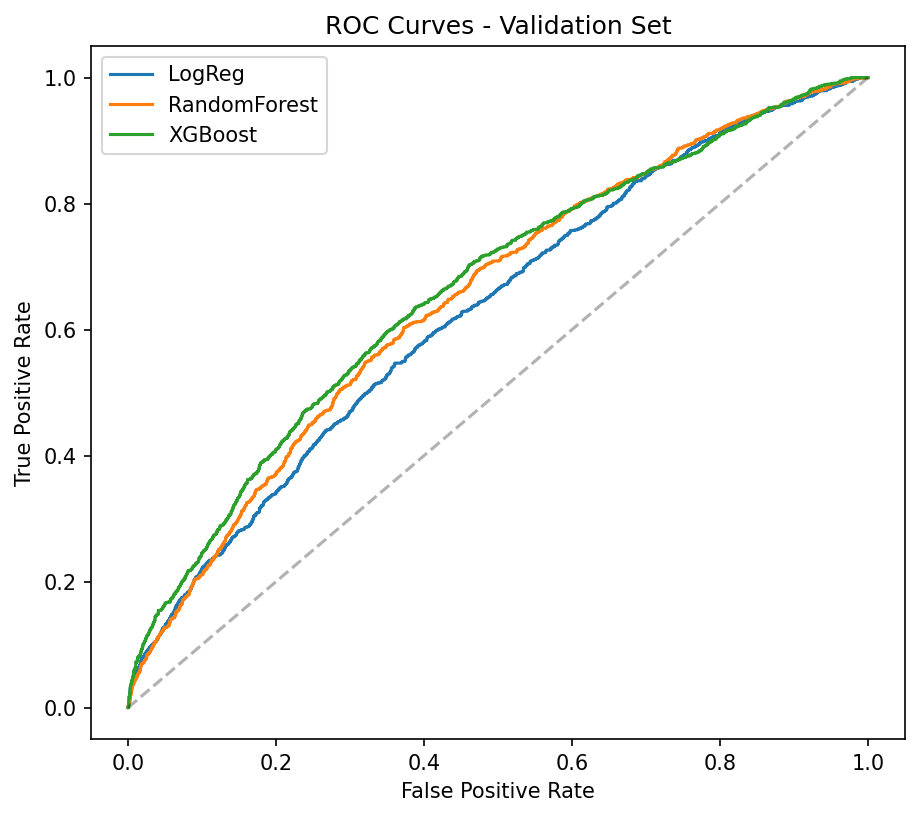
\includegraphics[width=0.72\textwidth]{plots/roc_curves_val.png}
\caption{Validation ROC curves for the evaluated models.}
\label{fig:roc}
\end{figure}

\subsection{Statistical Significance of Model Differences}
DeLong's test found no statistically significant AUROC difference among CatBoost, LightGBM, and XGBoost (CatBoost vs.\ LightGBM: $p=0.897$; CatBoost vs.\ XGBoost: $p=0.761$; LightGBM vs.\ XGBoost: $p=0.861$): the three models rank patients in a statistically indistinguishable manner. McNemar's test on paired binary decisions at a 0.5 threshold nevertheless revealed significant disagreement between CatBoost and LightGBM ($p<0.001$) and between CatBoost and XGBoost ($p<0.001$). This dissociation is clinically important: models that rank equally well can disagree substantially on which specific patients are flagged at a fixed operating threshold, so threshold selection and decision-level calibration deserve as much attention as headline AUROC.

\subsection{Calibration}
Temperature scaling (optimal $T=0.7494$) improved ECE from 0.3385 to 0.3257 and the Brier score from 0.2172 to 0.2156 (Table~\ref{tab:calibration}); the reliability diagram is shown in Fig.~\ref{fig:reliability}.

\begin{table}[!t]
\centering
\begin{threeparttable}
\caption{Calibration Before and After Temperature Scaling}
\label{tab:calibration}
\begin{tabular}{lcc}
\toprule
\textbf{Metric} & \textbf{Before} & \textbf{After} \\
\midrule
Expected calibration error & 0.3385 & 0.3257 \\
Brier score & 0.2172 & 0.2156 \\
Negative log-likelihood & 0.6239 & 0.6200 \\
\bottomrule
\end{tabular}
\begin{tablenotes}\footnotesize
\item Optimal temperature $T=0.7494$. Lower is better for all metrics.
\end{tablenotes}
\end{threeparttable}
\end{table}

\begin{figure}[!t]
\centering
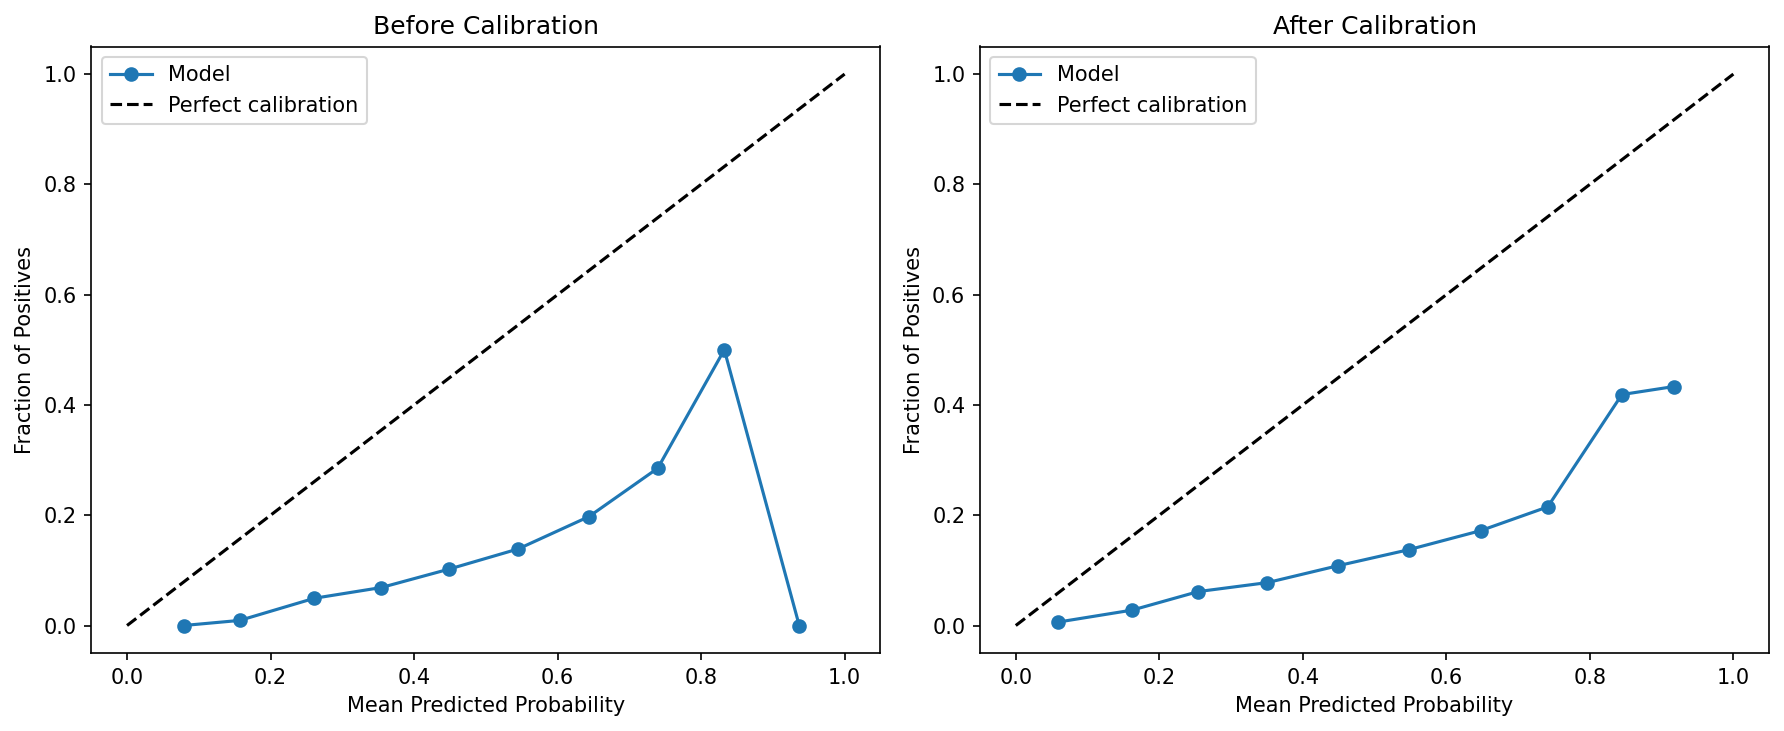
\includegraphics[width=0.72\textwidth]{plots/reliability_diagram.png}
\caption{Reliability diagram before and after temperature scaling.}
\label{fig:reliability}
\end{figure}

\subsection{Conformal Prediction}
At a target coverage of 90\%, empirical coverage on the held-out test set was 0.8969 with an average prediction-set size of 1.5838 (conformal quantile $\hat{q}=0.6684$), confirming near-nominal, distribution-free coverage.

\subsection{Explainability}
Global SHAP analysis (Fig.~\ref{fig:shap}) identified \emph{number\_inpatient} (mean $|$SHAP$|=0.241$), \emph{discharge\_disposition\_id} (0.197), and \emph{total\_prior\_visits} (0.097) as the top three predictors, consistent with clinical literature on healthcare utilization and discharge planning.

\begin{figure}[!t]
\centering
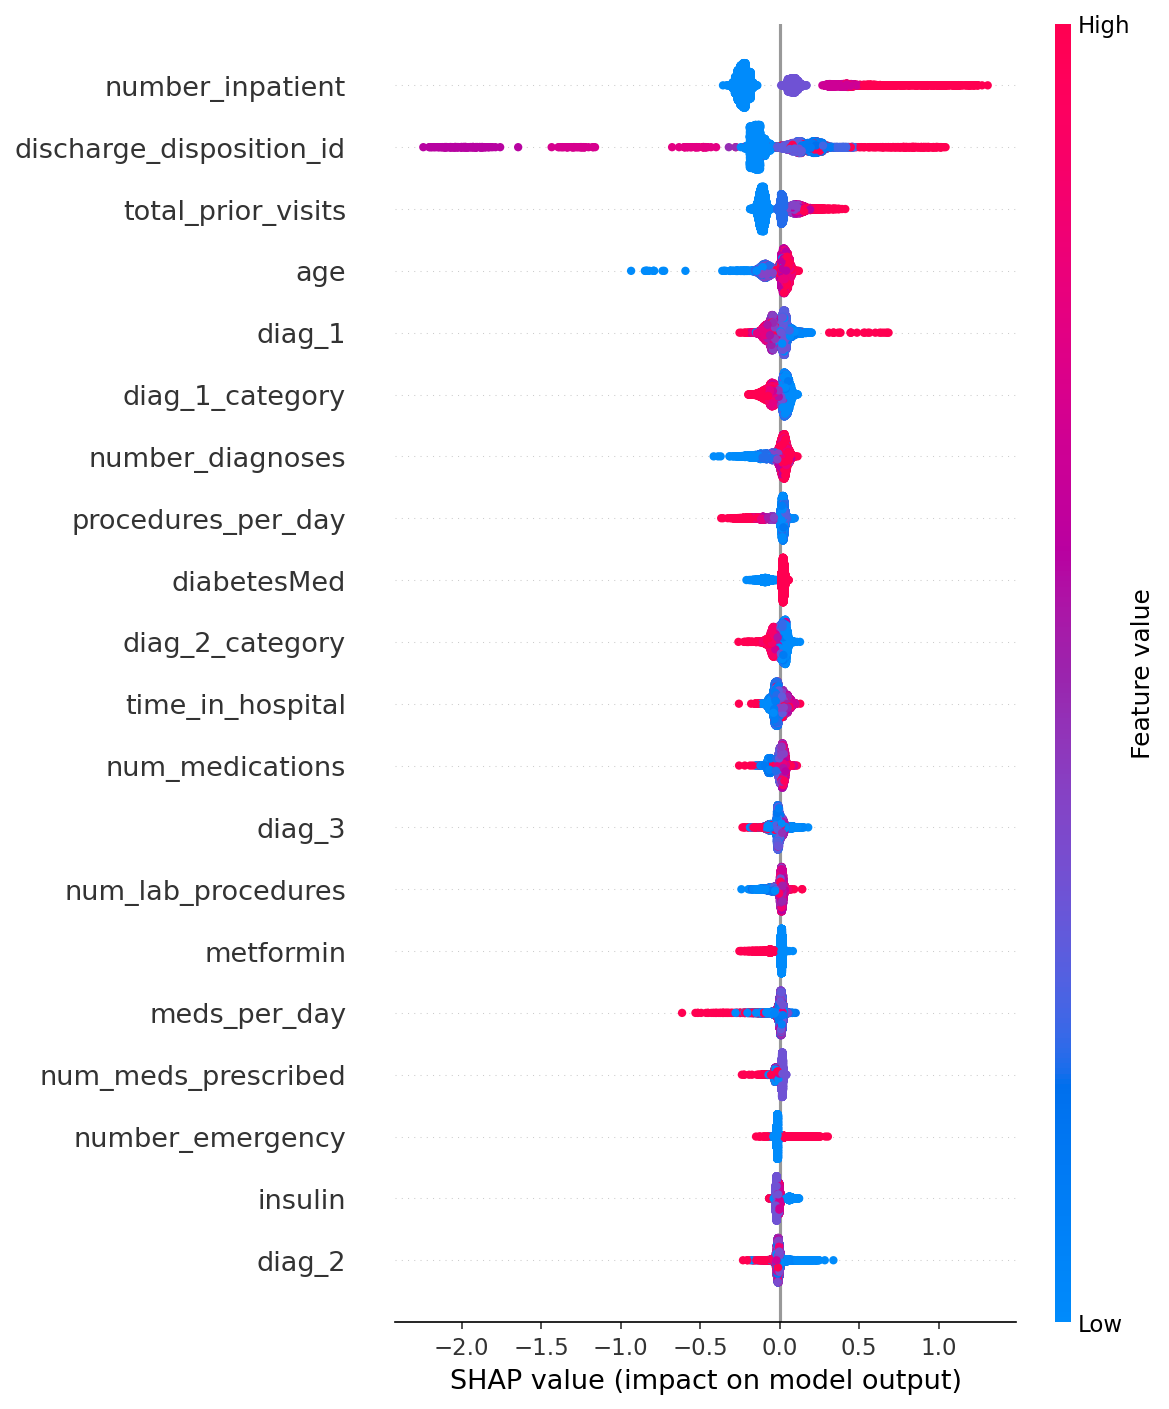
\includegraphics[width=0.62\textwidth]{plots/shap_summary_plot.png}
\caption{Global SHAP feature importance for the best model.}
\label{fig:shap}
\end{figure}

\subsection{Hallucination Refusal (Red-Team Test)}
When presented with fabricated, clinically irrelevant ``evidence,'' the explanation engine correctly declined to incorporate it, stating that the retrieved passage ``does not directly support or refute the identified risk factors,'' and explicitly flagged that the listed SHAP contributions were risk-lowering -- rather than generating a plausible but false justification. This behavior supports the claim that the system expresses genuine uncertainty rather than fabricating support.

\subsection{Fairness and Subgroup Analysis}
Table~\ref{tab:fairness} and Fig.~\ref{fig:fairness} summarize validation performance across race, gender, and age subgroups. Performance was comparable across the two largest race groups (Caucasian: AUROC 0.659, $n=7694$; African American: 0.654, $n=1843$); apparent differences in smaller subgroups (e.g., Asian, $n=54$) are likely artifacts of small sample size ($n<150$ for several groups) and should not be over-interpreted. Gender showed no meaningful disparity (female 0.660 vs.\ male 0.667). Age revealed a clinically meaningful pattern: discrimination was notably weaker for the oldest patients (80--90 years: AUROC 0.616; 90--100 years: 0.597) than for middle-aged patients (40--50 years: 0.745). Because elderly patients are both the largest and the highest-risk subgroup, this reduced reliability where accurate stratification matters most is a significant limitation warranting age-stratified modeling or elderly-specific features.

\begin{table}[!t]
\centering
\begin{threeparttable}
\caption{Subgroup Performance on the Validation Set}
\label{tab:fairness}
\begin{tabular}{lccc}
\toprule
\textbf{Subgroup} & $\boldsymbol{n}$ & \textbf{AUROC} & \textbf{AUPRC} \\
\midrule
\multicolumn{4}{l}{\emph{Race}} \\
Caucasian & 7694 & 0.6593 & 0.2160 \\
African American & 1843 & 0.6542 & 0.2096 \\
Unknown & 254 & 0.6969 & 0.1974 \\
Hispanic & 219 & 0.7465 & 0.3164 \\
Other & 145 & 0.7611 & 0.3055 \\
Asian & 54 & 0.8016 & 0.3584 \\
\midrule
\multicolumn{4}{l}{\emph{Gender}} \\
Female & 5460 & 0.6600 & 0.2082 \\
Male & 4749 & 0.6671 & 0.2319 \\
\midrule
\multicolumn{4}{l}{\emph{Age group (years)}} \\
10--20 & 76 & 0.7167 & 0.1635 \\
20--30 & 158 & 0.7364 & 0.2358 \\
30--40 & 370 & 0.7394 & 0.3202 \\
40--50 & 962 & 0.7451 & 0.3408 \\
50--60 & 1738 & 0.6884 & 0.2426 \\
60--70 & 2251 & 0.6438 & 0.1979 \\
70--80 & 2639 & 0.6381 & 0.2102 \\
80--90 & 1713 & 0.6160 & 0.1566 \\
90--100 & 289 & 0.5973 & 0.1676 \\
\bottomrule
\end{tabular}
\begin{tablenotes}\footnotesize
\item Estimates for subgroups with $n<150$ are unstable and should not be over-interpreted.
\end{tablenotes}
\end{threeparttable}
\end{table}

\begin{figure}[!t]
\centering
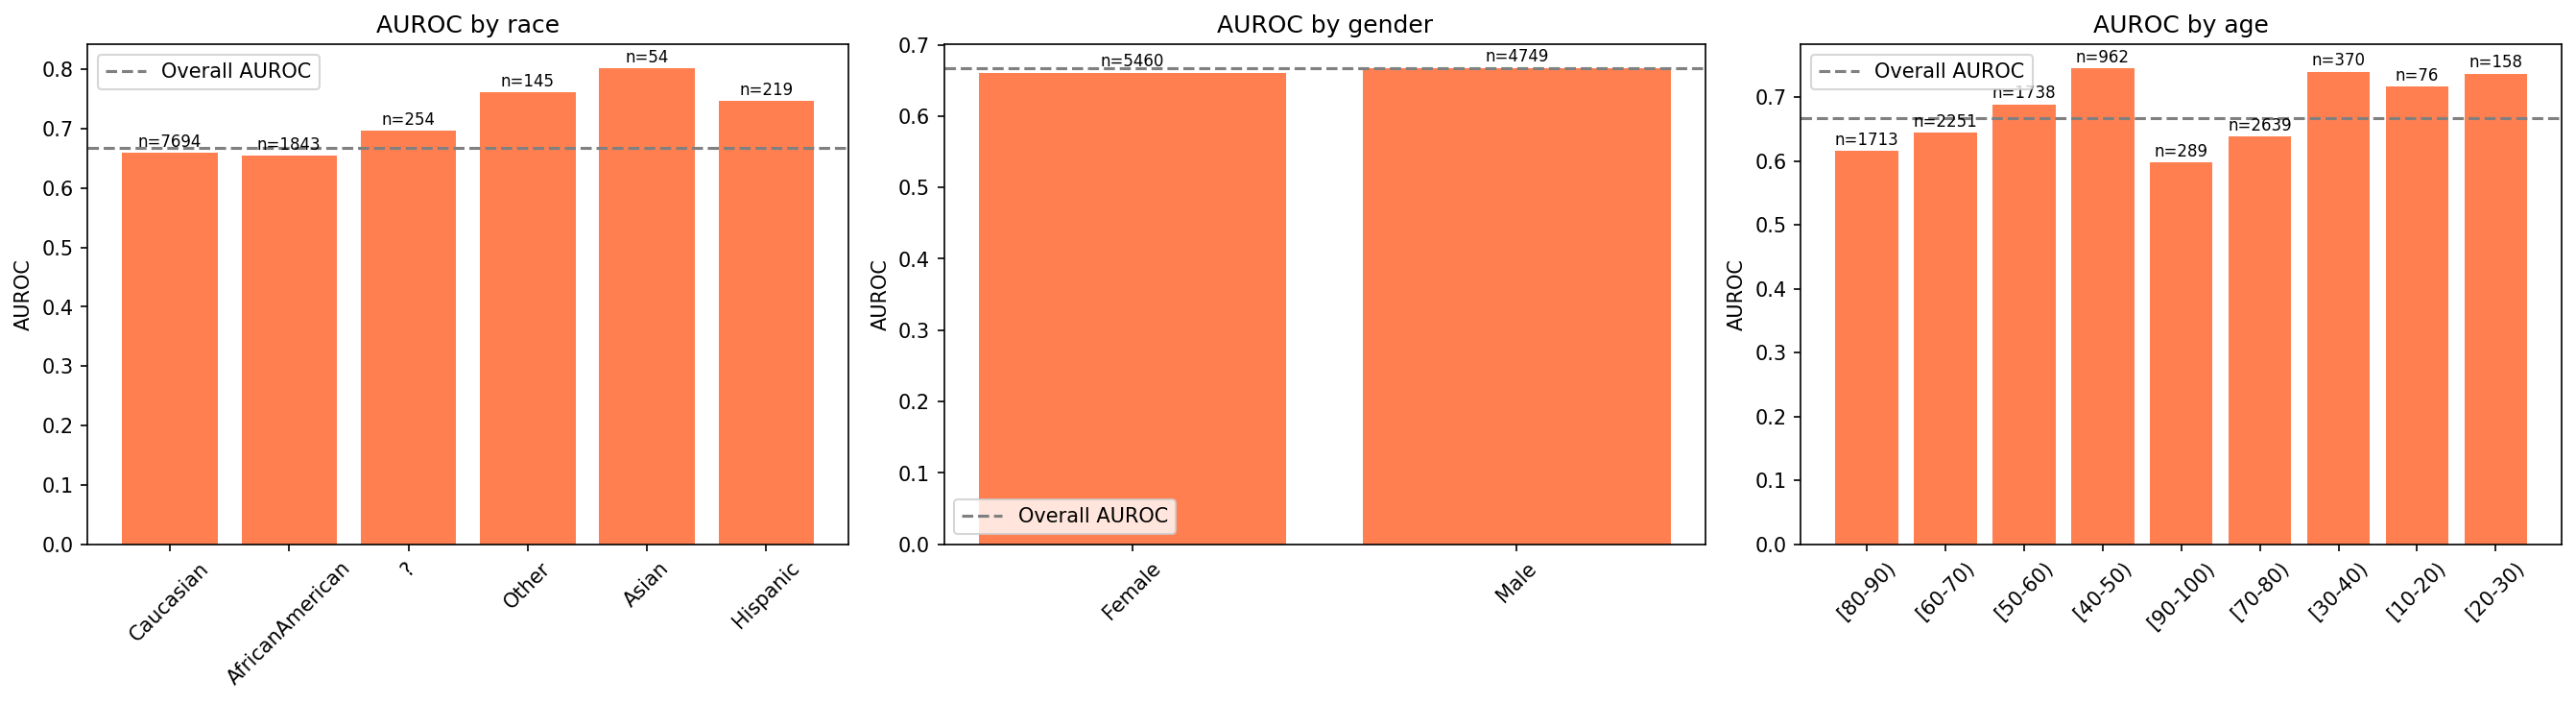
\includegraphics[width=0.85\textwidth]{plots/fairness_subgroup_auroc.png}
\caption{Validation AUROC across race, gender, and age subgroups.}
\label{fig:fairness}
\end{figure}

\section{Discussion}
\label{sec:discussion}
The AUROC ceiling of approximately 0.665--0.668 observed across gradient-boosted models is consistent with prior work on this dataset and reflects genuine limits of the predictive signal available from structured EHR fields alone: factors such as socioeconomic status and post-discharge support, known contributors to readmission risk, are absent from the data. Deep learning approaches did not outperform gradient-boosted trees, consistent with broader tabular benchmarks.

The dissociation between ranking ability and threshold-level agreement has direct deployment implications: because a single operating threshold must be chosen in practice, decision-level calibration and threshold selection deserve as much attention as discrimination when comparing candidate models.

Finally, the red-team result illustrates that coupling retrieval with an explicit refusal constraint yields explanations that degrade gracefully: when evidence is irrelevant, the system says so, instead of inventing support. We regard this ``capable of saying I don't know'' property as a necessary condition for trustworthy clinical decision support.

\section{Limitations}
\label{sec:limitations}
\begin{itemize}
    \item Predictive performance, while consistent with the literature, remains modest (AUROC $\approx 0.67$) and is not suitable for clinical deployment.
    \item The subgroup analysis is retrospective and unadjusted; small subgroups yield unstable estimates.
    \item The clinical evidence corpus used for retrieval is a small, illustrative, paraphrased set rather than a comprehensive guideline database.
    \item The dataset reflects clinical practice from 1999--2008 and may not generalize to current care patterns.
    \item The red-team evaluation is a single adversarial probe; broader stress-testing is needed.
\end{itemize}

\section{Ethics Statement}
\label{sec:ethics}
This system is a research prototype only and is explicitly not validated for clinical deployment. All system outputs carry disclaimers to this effect. No real patient data beyond the de-identified public dataset were used. Any real clinical decision must be made by a licensed healthcare professional using validated, approved clinical tools and their own clinical judgment.

\section{Conclusion}
\label{sec:conclusion}
TrustMedX demonstrates that combining calibrated uncertainty and retrieval-grounded explanation with standard machine learning and explainable AI produces a measurably more trustworthy clinical decision support output -- one capable of expressing ``I don't know'' as reliably as ``I know'' -- even when raw predictive accuracy is bounded by the limits of the available data. Future work includes richer data sources, an authoritative retrieval corpus, prospective validation, and mitigation of the identified age-related performance gap.

% NOTE TO AUTHOR: the entries in references.bib are placeholders generated
% from memory. Verify every author list, venue, volume and page range
% against the original publications before submission.
\bibliographystyle{IEEEtran}
\bibliography{references}

\end{document}